\documentclass{article}

\usepackage{url} 

\usepackage{pdfpages}
\usepackage{lastpage}
\usepackage{fancyhdr}
\usepackage{ngerman}


\usepackage{floatrow}
\usepackage[tableposition=top]{caption}
\floatsetup[table]{capposition=top}

\usepackage{amsmath, amssymb}

\usepackage[utf8]{inputenc}


\usepackage[numbib]{tocbibind}

%Gummi|065|=)
\title{Adiabatenkoeffizient}
\author{Johannes Winkler}
\date{}


\newcommand\twodigits[1]{%
   \ifnum#1<10 #1\else #1\fi
}



\lhead{Adiabatenkoeffizient}
\rhead{\today\\Johannes Winkler}
\cfoot{\twodigits{\thepage}~/ \pageref{LastPage}}

\begin{document}

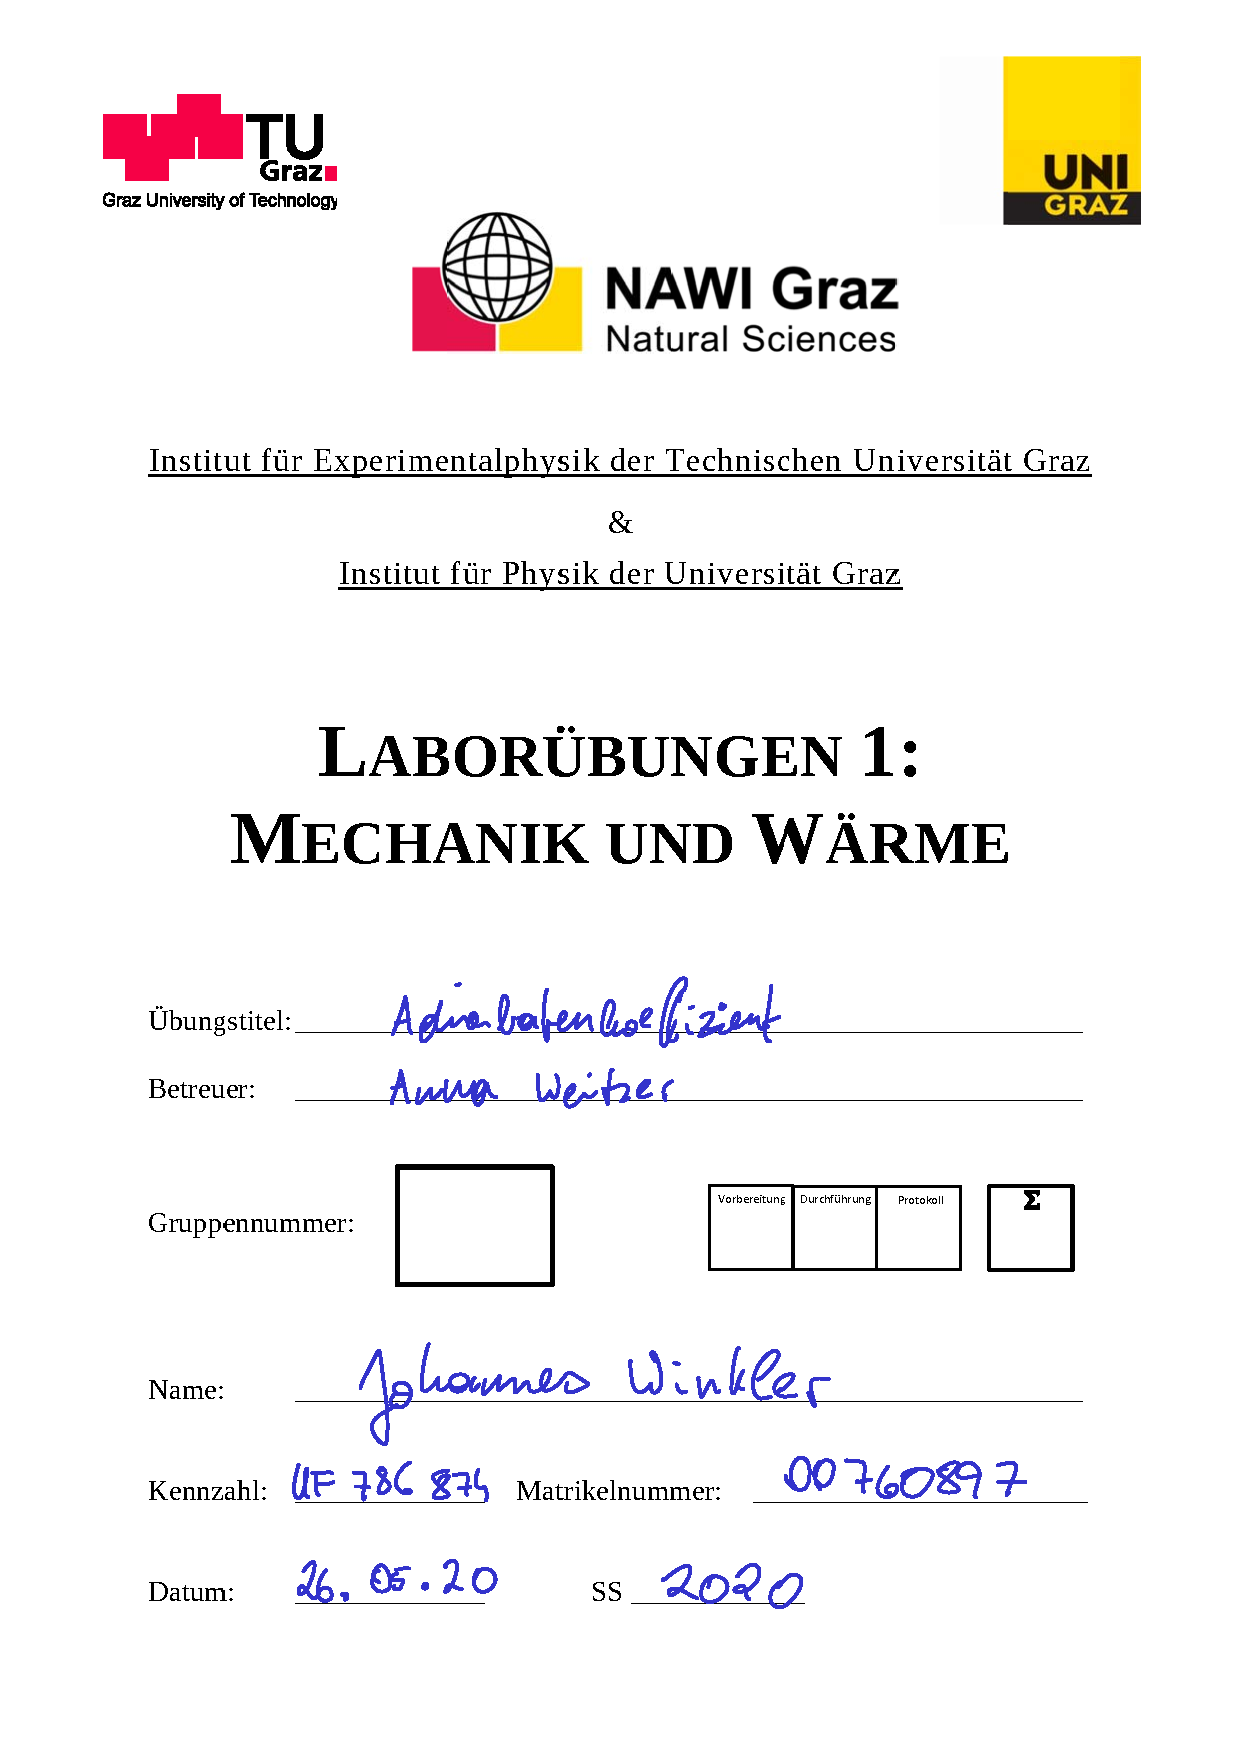
\includepdf[page=-]{deckblatt.pdf} 
 
 
\pagestyle{fancy}


\tableofcontents

\newpage


\section{Aufgabenstellung}

\begin{itemize}
\item Bestimmung des Adiabatenexponenten der Luft nach der Methode von Rüchardt.
\item Bestimmung des Adiabatenexponenten der Luft nach der Methode von Clement-Desormes.
\item Überprüfung der Methode nach Clement-Desormes auf systematische Fehler.
\end{itemize}



\section{Grundlagen}

\subsection{Methode nach Rüchardt}
Lässt man in einem nach oben offenen Präzisionsglasrohr mit der Querschnittsfläche $A$ (siehe Abbildung \ref{fig:pic1}) eine Kugel $K$ mit Masse $m$ fallen, so schwingt sie auf dem durch das abgeschlossene Volumen $V_0$ gebildeten Luftpolster mit der Periodendauer $\tau$. Da nur wenig Zeit für einen Wärmeaustausch mit der Umgebung zur Verfügung steht, wird die (De-)Kompression als adiabatisch angesehen. Aus der Differentialgleichung für eine ungedämpfte Schwingung ergibt sich für den Adiabatenexponenten
\begin{align}
\label{eq:kappa1}
\kappa = 4\cdot \pi^2 \cdot \frac{m\cdot V_0}{A^2\cdot p\cdot \tau^2}
\end{align}
wobei $p$ der Druck im Präzisionsglasrohr in der Nullposition der Kugel ist. Wird vom Barometer, das den Luftdruck auf Meereshöhe angibt, der Wert $p_0$ abgelesen, so ergibt sich unter Zuhilfenahme der barometrischen Höhenformel
\begin{align}
p = p_0 \cdot \exp\left(-\frac{h}{8000~\text{m}}\right) + \frac{m\cdot g}{A}
\end{align}
wobei die Seehöhe $h$ in Metern einzusetzen und $g = 9.81~\text{m s}^{-2}$ ist.

\subsection{Methode nach Clement-Desormes}

In eine Glasflasche (siehe Abbildung \ref{fig:pic2}) wird mit einem Blasbalg Luft eingepumpt. Nachdem sich die Temperatur in der Flasche an die Raumtemperatur angeglichen hat, wird der Überdruck $h_1$ (z.B. in mm Wasersäule) abgelesen. Wird der Hahn kurz geöffnet, so erfolgt der Druckausgleich (auf Labordruck) adiabatisch, wobei sich die eingeschlossene Luft abkühlt. Nach der anschließenden isochoren Erwärmung wird der Überdruck $h_2$ abgelesen. Aus den Gesetzen für adiabatische und isochore Zustandsänderungen ergibt sich der Adiabatenexponent zu
\begin{align}
\kappa = \frac{h_1}{h_1-h_2}
\end{align}
Dabei wurde vorausgesetzt, dass der Überdruck klein im Vergleich zum Luftdruck im Labor ist.




\section{Beschreibung der Versuchsanordnung}

\begin{figure}[h]

\begin{floatrow}
\ffigbox[\FBwidth]
{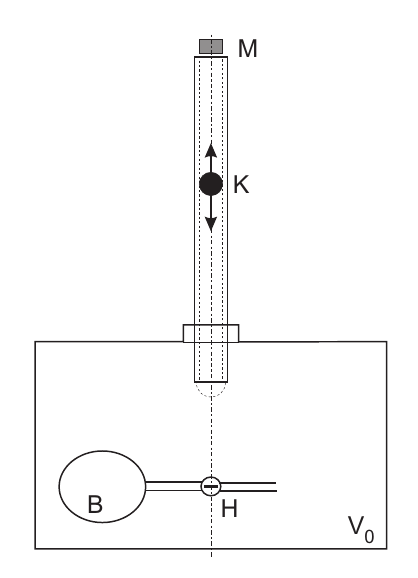
\includegraphics[height=5cm]{pic1.png}}
{\caption{Versuchsaufbau nach Rüchardt.
Das Gefäß mit Volumen $V_0$ kann mit dem
Blasbalg B aufgepumpt werden bis die Kugel K vom Magneten M gehalten wird. Durch
Öffnen von H wird der Druck auf Laborbedingungen ausgeglichen.
}
\label{fig:pic1}}

\ffigbox[\FBwidth]
{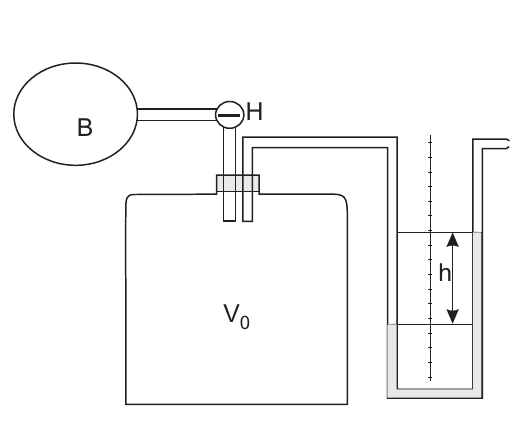
\includegraphics[height=5cm]{pic2.png}}
{\caption{Versuchsaufbau nach Clement-
Desormes. Mit dem Hahn H kann entweder
das Vorratsgefäß aufgepumpt (Blasbalg B) oder auf Labordruck gebracht werden. Der Überdruck wird über ein U-Rohrmanometer angezeigt.
}
\label{fig:pic2}}
\end{floatrow}

\end{figure}



\newpage
\section{Geräteliste}


Da aufgrund der Corona-Situation keine physische Anwesenheit im Labor möglich ist, können auch die genauen Serien- und Gerätenummern nicht angeben werden.

Da auch die Gebrauchsanleitung und Datenblätter der Werkzeuge nicht vorhanden sind, werden die Messfehler dieser Geräte geschätzt.


\begin{table}[h]
\caption{Geräteliste}

\begin{tabular}{lll}
Gerät  & Gerätenummer \\
\hline
Stoppuhr ($\Delta t = 0.1$~s) & axxxx \\
Blasbalg & bxxxx \\
Lichtschrankensensor & cxxxx \\
Kugel & dxxxx \\
Glasrohr & exxxx \\
U-Manometer & fxxxx \\
Glaskuppel & gxxxx \\
Lineal ($\Delta h=1$~mm) & hxxxx \\
Manometer ($\Delta p_0 = 20$~Pa) & ixxxx \\
Waage ($\Delta m = 0.05$~g) & jxxxx
\end{tabular}
\end{table}

\newpage
\section{Versuchsdurchführung und Messergebnisse}

\subsection{Methode nach Rüchardt}

Bei dieser Methode werden 5 Versuche durchgeführt, wobei die Zeit über mehrere Schwingungen gemessen und dann durch die Anzahl der Schwingungen dividiert wird. Dadurch erhalten wir näherungsweise die Dauer einer Schwingung~$\tau$. Die Unsicherheit für die Zeitmessung $\Delta t = 0.1~$s ist in diesem Fall ebenfalls durch die Schwingungsdauer zu dividieren. Also gilt für die Unsicherheit der Schwingungsdauer einer einzelnen Schwingung $\Delta \tau = 0.02~$s.

\begin{table}[H]
\caption{Messungen der Schwingungsdauer $\tau$}
\begin{tabular}{l|l}
Messung Nr. & $\tau$ / s \\
\hline
1 & 1.20 \\
2 & 1.14 \\
3 & 1.15 \\
4 & 1.15 \\
5 & 1.11 \\
\hline
$\overline{\tau}$ & 1.15
\end{tabular}
\end{table}


\subsection{Methode nach Clement-Desormes}

Hier wird der Druck in einem U-Manometer gemessen.

\begin{table}[H]
\caption{Messung der Höhen (angegeben in mm) im Manometer vor und nach dem Druckausgleich}
\label{tab:clement}
\begin{tabular}{l|lll|lll}
 & \multicolumn{3}{c|}{vorher}&  \multicolumn{3}{c}{nachher}\\
Messung Nr. & $h_l$ & $h_r$ & $\Sigma_v$ & $h_l$ & $h_r$ & $\Sigma_n$ \\
\hline
1 & 86 & 89 & 175 & 21 & 23 & 44 \\
2 & 93 & 95 & 188 & 21 & 21 & 42 \\
3 & 92 & 93 & 185 & 19 & 23 & 42 \\
4 & 90 & 91 & 181 & 21 & 22 & 43 \\
5 & 95 & 96 & 191 & 22 & 23 & 45 \\
\hline
$\overline{\Sigma}$ & & & 184 & & & 43.2
\end{tabular}
\end{table}

Für die Auswertung ist $\overline{\Sigma_v} = 184~$mm der durchschnittliche Abstand der Werte vor dem Druckausgleich und wird in der Formel als $h_1$ bezeichnet. Der durchschnittliche Abstand nach dem Druckausgleich wird als $h_2=43.2~$mm bezeichnet.

\newpage
\section{Auswertung}

\subsection{Bestimmung des Luftdruckes im Labor}
\label{subsec:druck}

Auf dem Barometer wurde $p_0=1008$~hPa abgelesen mit $\Delta p_0=20$~Pa. Aus \cite{graz} sieht man, dass Graz in einer Höhe von $h=353$~m über dem Meeresspiegel liegt, mit der Annahme, dass die Abweichung $\Delta h=10$~m beträgt. Zusätzlich ist die Masse $m=(16.73 \pm 0.05)$~g und die Querschnittsfläche abhängig von $d=(16.015 \pm 0.002)$~mm angegeben. In die gegebene Formel eingesetzt ergibt das
\begin{align}
p &= p_0 \cdot \exp\left(-\frac{h}{8000~\text{m}}\right) + \frac{4\cdot m\cdot g}{d^2\cdot \pi} \\
p &= 100800 \cdot \exp\left(-\frac{353~\text{m}}{8000~\text{m}}\right) + \frac{4\cdot 0.01673\cdot 9.81}{0.016^2\cdot \pi} = 972.64~\text{hPa}
\end{align}
Für die Unsicherheit ergibt sich
\begin{align}
\Delta p &= \left| \frac{\partial p}{\partial p_0} \right| \cdot \Delta p_0 + \left| \frac{\partial p}{\partial h} \right| \cdot \Delta h+\left| \frac{\partial p}{\partial m} \right| \cdot \Delta m + \left| \frac{\partial p}{\partial d} \right| \cdot \Delta d  \\
&= \Delta p_0 \cdot \exp\left(-\frac{h}{8000~\text{m}}\right) +p_0\cdot\exp\left(-\frac{h}{8000~\text{m}}\right)\cdot \frac{\Delta h}{8000~\text{m}}
 \\
\nonumber &+ \frac{4\cdot \Delta m\cdot g}{d^2\cdot \pi} + \frac{8\cdot m\cdot g \cdot \Delta d}{d^3\cdot \pi} \\
&= \exp\left(-\frac{h}{8000~\text{m}}\right)\cdot \left( \Delta p_0 + \frac{p_0\cdot \Delta h}{8000~\text{m}}\right) + \frac{4\cdot g}{d^2\cdot \pi}\cdot \left(\Delta m + \frac{2\cdot m\cdot \Delta d}{d} \right) \\
&= 142.3363~\text{Pa}
\end{align}
Der Luftdruck ist daher
\begin{align}
p = (972.64 \pm 1.42)~\text{hPa}.
\end{align}
\subsection{Methode nach Rüchardt}


Der Adiabatenkoeffizient ist in Gleichung \eqref{eq:kappa1} definiert wobei $A=d^2/4\cdot \pi$ die Querschnittsfläche der Glassäule ist, mit $d=(16.015 \pm 0.002)$~mm. Für die Masse der Kugel gilt $m=(16.73 \pm 0.05)$~g. Für den Adiabatenkoeffizienten und dessen Unsicherheit gilt nun

\begin{align}
\kappa &= 4\cdot \pi^2 \cdot \frac{m\cdot V_0}{\left(d^2/4\cdot \pi\right)^2\cdot p\cdot \tau^2} \\
\kappa &= 64\cdot \frac{m\cdot V_0}{d^4\cdot p\cdot \tau^2} 
\end{align}
\begin{align}
\Delta \kappa &= \left| \frac{\partial \kappa}{\partial m} \right| \cdot \Delta m + \left| \frac{\partial \kappa}{\partial d} \right| \cdot \Delta d + \left| \frac{\partial \kappa}{\partial p} \right| \cdot \Delta p + \left| \frac{\partial \kappa}{\partial \tau} \right| \cdot \Delta \tau \\
\Delta \kappa &= 64\cdot V_0\cdot  \left( \frac{\Delta m}{d^4\cdot p\cdot \tau^2} + \frac{4\cdot m\cdot\Delta d}{d^5\cdot p\cdot \tau^2} + \frac{m\cdot \Delta p}{d^4\cdot p^2\cdot \tau^2} + \frac{2\cdot m\cdot\Delta\tau}{d^4\cdot p\cdot \tau^3} \right) \\
\Delta \kappa &= \frac{64\cdot V_0}{d^4\cdot p\cdot \tau^2}\cdot \left( \Delta m + 4\cdot m\cdot \frac{\Delta d}{d} + m\cdot \frac{\Delta p}{p} + 2\cdot m\cdot \frac{\Delta \tau}{\tau}\right) \\
\end{align}
Hier wurde für $V_0 = 0.011$~m${}^3$, $m=(16.73\pm0.05)$~g und $d=(16.015\pm0.002)$~mm eingesetzt. Zusätzlich wurden $p$ und $\Delta p$ aus Abschnitt \ref{subsec:druck} verwendet.
\begin{align}
\Delta \kappa &= \frac{110.03}{\tau^2}\cdot \left(8.2\cdot 10^{-5} + 0.03\cdot \frac{\Delta \tau}{\tau}\right) \\
\Delta \kappa &= \frac{3.6816}{\tau^2}\cdot \left(2.47579\cdot 10^{-3} + \frac{\Delta \tau}{\tau}\right)
\end{align}

Damit lässt sich die Unsicherheit von $\kappa$ für gegebene $\tau$ und $\Delta \tau$ berechnen.

Bei einer mittleren Schwingungsdauer von $\tau=1.15$~s und einer geschätzten Abweichung $\Delta \tau = 0.02$~s erhält man
\begin{align}
\kappa &= 1.39 \\
\Delta \kappa &= 0.06
\end{align}



\subsection{Methode nach Clement-Desormes}

Hier ist der Adiabatenindex
\begin{align}
\kappa = \frac{h_1}{h_1-h_2}
\end{align}
und dessen Unsicherheit ist
\begin{align}
\Delta \kappa &= \left| \frac{\partial\kappa}{\partial h_1}\right|\cdot \Delta h_1 + \left| \frac{\partial\kappa}{\partial h_2}\right|\cdot \Delta h_2 \\
&= \frac{\Delta h_1 \cdot h_2}{(h_1-h_2)^2} + \frac{h_1\cdot \Delta h_2}{(h_1-h_2)^2}
\end{align}
Die Unsicherheit einer einzelnen gemessenen Höhe beträgt $\Delta h_1 = \Delta h_2 = 1$~mm. Da in Tabelle \ref{tab:clement} immer zwei gemessene Höhen addiert werden, verdoppeln sich die Unsicherheiten. Die Reduzierung nach der Abweichung gemäß zentralem Grenzwertsatz wird zugunsten von Messfehlern vernachlässigt. Somit ergibt sich als Gesamtfehler für Höhen $\Delta h = 2\cdot \Delta h_1 = 2~$mm.
\begin{align}
\Delta \kappa &= \Delta h \cdot\frac{h_1 + h_2}{(h_1-h_2)^2}
\end{align}

Durch Einsetzen von $h_1=184$~mm und $h_2 = 43.2$~mm und der Messunsicherheit ergibt sich
\begin{align}
\kappa &= 1.31 \\
\Delta \kappa &= 0.03
\end{align}


\newpage
\section{Zusammenfassung und Diskussion}

Für die Rüchardt Methode ergab sich
\begin{align}
\kappa &= 1.39 \pm 0.06
\end{align}

Die Clement-Desormes Methode ergab
\begin{align}
\kappa &= 1.31 \pm 0.03
\end{align}

Wenn man dies mit Literatur wie \cite{demtr1} oder \cite{giancoli} vergleicht, sieht man, dass die Methode nach Rüchardt genauer an dem in der Literatur erwarteten Wert liegt. Die Methode von Clement-Desormes liegt hingegen auch mit der berechneten Unsicherheit weit von den Literaturwerten entfernt. Es lässt sich daher darauf schließen, dass es bei dieser Methode möglicherweise eine systematische Abweichung gibt.


Rechnerisch interessant an diesem Beispiel ist die Tatsache, dass die eingesetzten Einheiten in die Formel nach Clement-Desormes egal sind, sofern konsistent immer dieselbe Einheit verwendet wird. Dies liegt an der Dimensionslosigkeit der Größe $\kappa$ und daran, dass nur Längen eingesetzt werden.


Zusammengefasst lässt sich sagen, dass die Methode nach Rüchardt genauer ist. Als Ursache kann man sagen, dass sich bei der zweiten Methode die Säulen im Manometer langsam bewegen und dass der Wert möglicherweise zu früh abgelesen wird. Zusätzlich wird vorausgesetzt, dass der Überdruck klein im Vergleich zum Druck im Labor ist. Dies könnte ebenfalls zu Ungenauigkeiten führen. Weitere Quellen für Unsicherheit sind möglicherweise undichte Stellen, oder Verdunstung von Wasser.




\begin{thebibliography}{9}
\bibitem{demtr1} W. Demtröder, \emph{Experimentalphysik 1: Mechanik und Wärme}, Springer-Spektrum, 8. Auflage, 2018.

\bibitem{giancoli} D. Giancoli, \emph{Physik}, Pearson, 4. Auflage, 2019.

\bibitem{graz} \url{https://de.wikipedia.org/wiki/Graz} (Stand: \today)


\end{thebibliography}

\end{document}
